\subsection{Level3.3: 任意の評価用データを用いた評価}
\subsubsection{アプローチ}
(仮説1)\\
学習時のデータ(教師データ)との違いが少ない程認識率が高く、
逆に教師データとの違いが多い程認識率が低くなるとの仮定の下、
如何に示す評価データを用意した。
\begin{itemize}
	\item a\_deter1.txt
	\item a\_deter2.txt
	\item a\_deter3.txt
	\item a\_deter4.txt
	\item a\_deter5.txt
	\item a\_deter6.txt
\end{itemize}

 (仮説2) \\
 学習時のデータ(教師データ)との違いが多い程認識率が高く、
 逆に教師データとの違いが少ない程認識率が低くなるとの仮定の下、
 評価データは仮説1と同様のものを用いる。

(仮説3)\\
学習データの一部分だけの場合,一部分が似ているものの認証率が高いという仮定の下,
「あ」のデータを上下左右の半分だけのデータを用意した.また他の文字の左半分だけのデータも用意した.
\begin{itemize}
	\item a\_up.txt
	\item a\_down.txt
	\item a\_left.txt
	\item a\_half.txt 
	\item ka\_half.txt
	\item sa\_half.txt
	\item ta\_half.txt
	\item na\_half.txt
	\item ha\_half.txt
	\item ma\_half.txt
	\item ya\_half.txt
	\item ra\_half.txt
	\item wa\_half.txt
\end{itemize}


\subsubsection{結果}
\begin{figure}[h]
 \begin{center}
  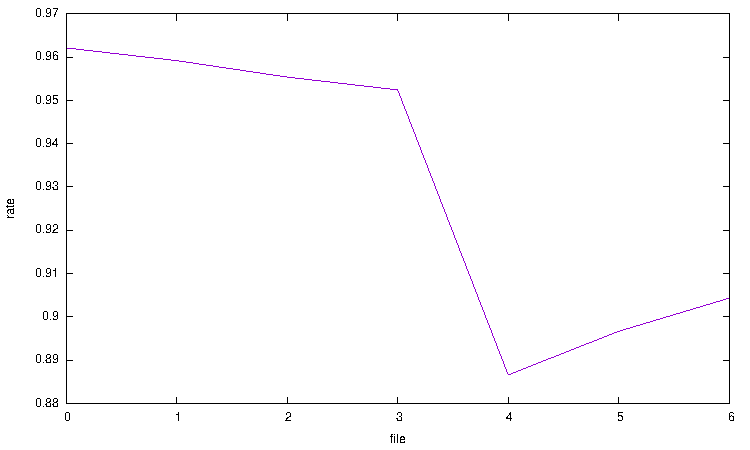
\includegraphics[width=10.0cm]{figs/level3/deter.pdf}
  \caption{仮説1:認証率(rate)と違い}
  \label{fig:level3_3_1}
 \end{center}
\end{figure}
上記のX軸は,0が学習データと同じデータ,1以降はa\_deter.txtの番号となっている.またこの番号が上がるにつれて,元データよりデータを劣化(1-$>$0)にしている.

\begin{figure}[h]
 \begin{center}
  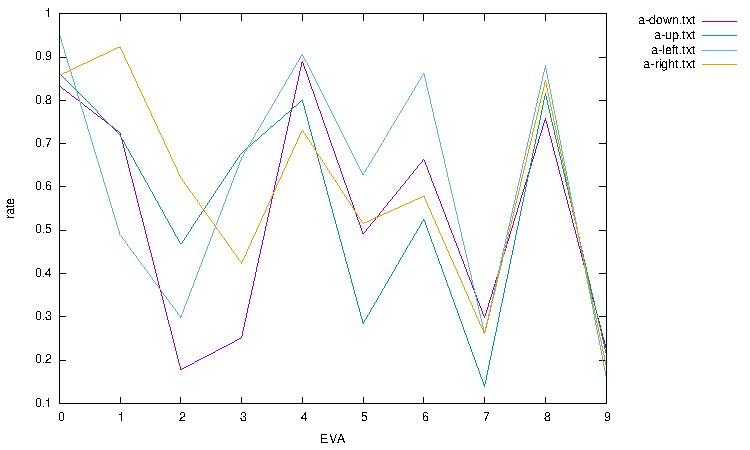
\includegraphics[width=10.0cm]{figs/level3/adata.pdf}
  \caption{仮説3:「あ」のデータ}
  \label{fig:level3_3_2}
 \end{center}
\end{figure}

\begin{figure}[h]
 \begin{center}
  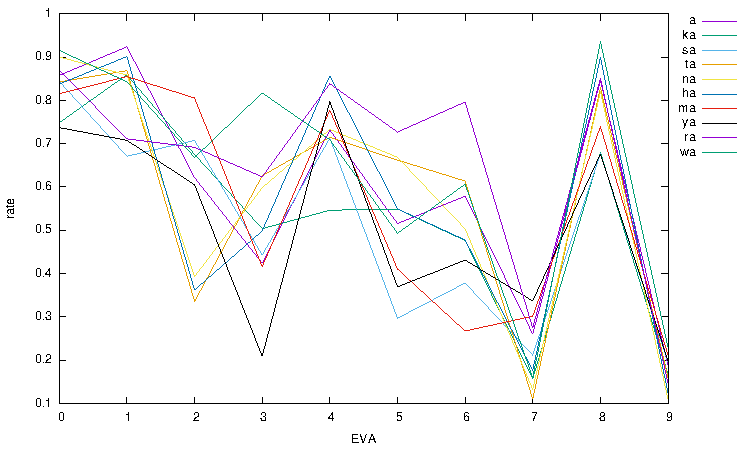
\includegraphics[width=10.0cm]{figs/level3/mozi.pdf}
  \caption{仮説3:学習データすべての半分}
  \label{fig:level3_3_3}
 \end{center}
\end{figure}

\subsubsection{考察}
結果として
\begin{itemize}
	\item 仮説1,2: 違いが増えるほど認証率は低くなるが,ほとんどデータを劣化させた場合少し高くなる.
	\item 仮説3: 「あ」のデータを移動させた場合,「あ」としての認証率が高く,他にも「な」や「ら」,「か」などの文字としての認証率も高かった.
	\item 仮説3: 学習データ全ての文字を半分にしてみた場合,「あ」,「か」,「な」,「ら」の認証率が高かった.
\end{itemize}
というデータを得た.\\
図\ref{fig:level3_3_1}のデータの中で,ほとんどデータを劣化させたa\_deter5.txtとa\_deter6.txtの認証率が若干高くなったのは,ほとんどデータが少なく判断できなかったことで全体的に認証率が上がったのではないかと推測する.\\
図\ref{fig:level3_3_2},\ref{fig:level3_3_3}より,似た部分の多い「あ」,「か」,「な」,「ら」の4つの認証率が高いことがわかった.\\
よって,仮説1と3が正しいという結果になった.
